\chapter{Tool Analysis: Existing Approaches to Container Energy Consumption}
\label{chap:tool-analysis}

\section{Introduction}
\label{sec:tool-intro}

\section{Non-container-focused Energy Monitoring Tools}
\label{sec:non-k8s-tools}
\subsection{Server-Level Energy Monitoring}
\label{sec:server-tools}
While not directly translatable to container-level energy monitoring, server-level energy consumption is an important aspect of it. Scientific works and tools in this domain generally don't provide the temporal resolution required for container-level energy monitoring.

\subsubsection{Kavanagh and Djemame: Energy Modeling via IPMI and RAPL Calibration}
\label{sec:kavanagh}

\paragraph{Overview and Architecture}
Kavanagh and Djemame\parencite{kavanagh2019rapid} present their findings on combining IPMI and RAPL (interface unspecified) data to estimate server energy consumption, achieving improved accuracy through calibration with an external server-level Watt meter. For calibration, they induce artificial CPU workloads and rely on CPU utilization metrics with 1-minute averaging windows, necessitating extended calibration intervals to obtain stable readings. While the resulting model is tailored to their specific hardware and not generally portable, their work provides valuable insights into the complementary use of IPMI and RAPL. The authors recognize that the respective limitations of these tools (RAPL’s partial scope and IPMI’s low resolution) can be mitigated when used in combination.

\paragraph{Attribution Method and Scope}
Although the model operates at the physical host level, it supports attribution to VMs or applications using CPU-utilization-based proportional allocation. Several allocation rules are proposed, including utilization ratio, adjusted idle sharing, and equal distribution. However, no container-level attribution is attempted, and runtime flexibility is limited due to the static nature of the calibration.

\paragraph{Validation and Limitations}
With their Watt-meter-calibrated model using segmented linear regression, the authors report an average error of just -0.17\%. More relevant to practical application, they also construct a model based solely on IPMI and RAPL(calibrated via Watt meter data) which achieves a reduced error of -5.58\%, compared to -15.75\% without calibration. Limitations of their approach include the need for controlled, synthetic workloads, coarse-grained sensor input, and the assumption of relatively stable system conditions during calibration.

\paragraph{Key Contributions}
\begin{itemize}
    \item \textbf{Hybrid use of IPMI and RAPL is analyzed}, showing that these tools compensate for each other’s limitations. RAPL underestimates total system power, while IPMI captures more components but at lower resolution.
    \item IPMI accuracy is significantly improved through external Watt meter calibration.
    \item The authors provide practical calibration guidelines:
    \begin{itemize}
        \item Use long, static workload plateaus to align with averaging windows and reduce synchronization complexity.
        \item Discard initial and final measurement intervals to avoid transient noise and averaging artifacts.
        \item Ensure calibration workloads exceed the IPMI averaging window to capture valid steady-state values.
    \end{itemize}
\end{itemize}

\paragraph{Relevance to Proposed Architecture}
This work informs the proposed architecture by demonstrating how combining RAPL and IPMI can yield more accurate system-level power estimation. The use of plateau-based calibration and composite data models is especially applicable. However, the lack of container-level granularity, reliance on offline calibration, and limited attribution scope underscore the need for more dynamic, fine-grained, and container-aware approaches in Kubernetes-based environments.

\subsubsection{CodeCarbon}
CodeCarbon\parencite{codecarbon_2024} is a Python package designed to estimate the carbon emissions of a program’s execution. While its implementation is general-purpose, it is primarily aimed at machine learning workloads.

\paragraph{Overview and Architecture}
CodeCarbon estimates a workload’s energy consumption by relying on RAPL \textit{package-domain} CPU metrics via the \texttt{powercap} RAPL file system interface. A fix for the RAPL MSR overflow issue was implemented\parencite{codecarbon_issue_322}. In the absence of RAPL support, it falls back to a simplified model based on the CPU’s Thermal Design Power (TDP), obtained from an internal database, and combines it with CPU load metrics from \texttt{psutil}. For memory, a static power value is assumed based on the number and capacity of installed DIMMs. GPU power consumption is estimated via NVIDIA’s NVML interface. The default measurement interval is 15 seconds, with the authors citing lightweight design as the primary motivation.

The component-level estimations are then aggregated and multiplied by a region-specific net carbon intensity (based on the local electricity grid’s energy mix) to estimate the program’s total CO\textsubscript{2} emissions. CodeCarbon is typically executed as a wrapper around code blocks, scripts, or Python processes.

\paragraph{Limitations}
There is no direct attribution of CPU activity to individual power metrics: CodeCarbon estimates energy use indirectly, based on the number of active cores and average CPU utilization, while making many assumptions that could be prevented. Combined with the relatively long measurement intervals, this results in background system processes also being attributed to the measured Python program. Consequently, CodeCarbon does not contribute directly to the goals of this thesis, which seeks fine-grained, container-level attribution.

However, the tool highlights several interesting secondary considerations. The integration of regional CO\textsubscript{2} intensity data is a valuable extension to conventional energy measurement and is well implemented. Additionally, the Python-based design offers high accessibility and ease of use, which may serve as inspiration for future developer-facing tools.

\subsubsection{AI Power Meter}
\textit{AI Power Meter}\parencite{aipowermeter} is a lightweight Python-based tool designed to monitor the energy consumption of machine learning workloads. It gathers power consumption data for the CPU and RAM via Intel RAPL using the \texttt{powercap} interface, and for the GPU via NVIDIA’s NVML library. While the authors acknowledge that other system components (e.g., storage, network) also contribute to energy usage, these are not currently included and are considered an accepted limitation of the tool.

Unlike more advanced attribution tools, AI Power Meter does not distinguish between individual processes or workloads. Instead, it provides coarse-grained, system-level energy consumption measurements over time. In this respect, its scope is similar to \textit{CodeCarbon}, focusing on ease of use and integration into ML pipelines rather than precise, per-process energy attribution. As such, while not directly applicable to container-level measurement or power attribution, AI Power Meter demonstrates the growing interest in accessible energy monitoring tools within the machine learning community.

\subsection{Telemetry-Based Estimation Frameworks}
\label{sec:telemetry-tools}

\subsubsection{PowerAPI Ecosystem\parencite{powerapi2024github} (PowerAPI, HWPC, SmartWatts)}
\label{sec:powerApiFramework}

PowerAPI\parencite{fieni2024powerapi} is an open-source middleware toolkit for assembling software-defined power meters that estimate real-time power consumption of software workloads. Developed as a generalized and modular framework, PowerAPI evolved alongside specific implementations such as \textit{SmartWatts}, detailed in section~\ref{sec:smartwatts}. It allows power attribution at multiple granularity levels, including processes, threads, containers, and virtual machines. A distinctive strength of PowerAPI is the continuous self-calibration of its power models, enabling accurate real-time energy estimation under varying workloads and execution conditions. This makes PowerAPI particularly suited to heterogeneous computing infrastructures.

\paragraph{Overview and Architecture}

PowerAPI uses an actor-based model for modularity, enabling easy customization of its internal components with minimal coupling. It supports raw metric acquisition from diverse sensors (e.g., physical meters, processor interfaces, hardware counters, OS counters) and delivers power consumption data through various output channels (including files, network sockets, web interfaces, and visualization tools). As middleware, PowerAPI facilitates assembling power meters "\textit{à la carte}" to accommodate specific user requirements and deployment scenarios.

\paragraph{Core Components}
\begin{itemize}
    \item \textbf{powerapi-core}: Middleware orchestrating real-time/post-mortem interactions between sensors and formulas. It defines the essential interfaces for sensor data ingestion and output channels (e.g., MongoDB, InfluxDB, CSV, socket, Prometheus), and includes built-in capabilities for data preprocessing, postprocessing, and reporting.
    \item \textbf{hwpc-sensor}: A telemetry probe designed to gather low-level hardware performance counters (HWPCs), including instructions, cycles, and RAPL energy metrics. This sensor leverages \textit{perf} and \textit{cgroups-v2}, critical for fine-grained telemetry in containerized environments. It also provides detailed CPU performance state metrics via MSR events (\texttt{TSC}, \texttt{APERF}, \texttt{MPERF}).
    \item \textbf{SmartWatts-formula}\parencite{fieni2020smartwatts}: A power model implementation (in Python) using HWPC data to estimate power consumption dynamically. It employs online linear regression provided by the Python \textit{scikit-learn}\parencite{scikit-learn} library, enabling accurate runtime learning of workload-specific power signatures. SmartWatts is further detailed in section~\ref{sec:smartwatts}.
    \item \textbf{SelfWatts-controller}: Dynamically selects hardware performance counters for software-defined power models, facilitating automatic configuration and unsupervised deployment in heterogeneous infrastructures. Currently, its development has stalled for several years, limiting its practical applicability.
    \item \textbf{pyRAPL}: A convenient Python wrapper around RAPL for CPU, DRAM, and iGPU energy metrics collection, providing easy access to hardware-based power data.
\end{itemize}

\paragraph{Relevance and Integration}
The modular and extensible architecture of PowerAPI positions it as a highly suitable foundation for further research and development of specialized power attribution tools. Researchers can readily extend or adapt its components to address evolving or niche requirements. However, its current implementation does not incorporate certain critical metrics, such as IPMI-based telemetry, which could limit its completeness in some practical deployment scenarios. Nonetheless, PowerAPI represents a significant advancement toward the creation of generalized, plug-and-play power models that operate without extensive manual calibration. This emphasis on practical deployability and general applicability highlights a key strength of the project and sets a clear direction for future research and development efforts in the domain of software-defined energy monitoring.

\subsubsection{Green Metrics Tool}

The \textit{Green Metrics Tool} (GMT)\parencite{greencodingdocs} is an open-source framework designed to measure the energy consumption of containerized applications across various phases of the software lifecycle, including installation, boot, runtime, idle, and removal. It uses small, modular metric collectors to gather host-level energy and system data (e.g., CPU and DRAM energy via RAPL, IPMI power readings), and is orchestrated through declarative usage scenarios.

While GMT provides reproducible, lifecycle-aware measurements in controlled environments, it does \textit{not} perform container-level or process-level energy attribution. The developers explicitly avoid splitting energy consumption across containers, citing the lack of reliable attribution models.

\section{Container-Focused Energy Attribution Tools}
\label{sec:container-tools}


































































\subsection{Kepler}
\label{sec:kepler}
%\parencite{kepler_energy} -> KEPLER repo
%\parencite{amaralKeplerFrameworkCalculate2023} -> KEPLER paper
%\parencite{pijnackerEstimatingContainerlevelPower2024} -> Pijnacker Master thesis
%\parencite{pijnackerContainerlevelEnergyObservability2025} -> Pijnacker official paper
%\parencite{choochotkaewAdvancingCloudSustainability2023} -> "Advancing Cloud Sustainability: A Versatile Framework for Container Power Model Training"
%    --> not really relevant, this is about using KEPLER for modeling of static power if RAPL is NOT available (i.e. in cloud)
%\parencite{amaral2023exploring} -> article about kepler, st
%
%https://www.green-coding.io/case-studies/cpu-utilization-usefulness/: Let’s now make another approach though not using CPU utilization, but rather by using CPU instructions, which is the same technique as for instance Kepler uses



\subsubsection{Overview and Goals}
\label{sec:kepler-overview}

Kepler (\textit{Kubernetes-based Efficient Power Level Exporter})\parencite{kepler_energy} is a modular, Kubernetes-native framework for monitoring, modeling, and estimating energy consumption in containerized environments. As the most prominent tool for container-level power estimation in Kubernetes, Kepler enables detailed observability of energy usage at the level of individual processes, containers, pods, and nodes\parencite{amaralKeplerFrameworkCalculate2023}.

Kepler integrates seamlessly with Kubernetes and Prometheus-based observability stacks. It supports both real-time energy metrics (e.g., RAPL, ACPI, NVML) and model-based estimation through trained regression models, making it applicable across a wide range of deployment environments, from bare-metal servers to virtual machines. Developed as an open-source CNCF project, Kepler’s architecture is designed to be extensible, allowing researchers and practitioners to contribute new power models and adapt it to diverse system architectures.

\subsubsection{Architecture and Metric Sources}
\label{sec:kepler-architecture}

Kepler's architecture consists of several interconnected components, with the core functionality centered around a privileged monitoring agent that runs on every node. While the framework supports model-based estimation for environments without hardware telemetry, this thesis focuses on the direct collection of real-time power and utilization metrics available in bare-metal deployments.

\paragraph{Deployment Models}
Kepler supports multiple deployment scenarios depending on the availability of energy sensors on the host system. In bare-metal environments, Kepler can directly collect power metrics using RAPL, ACPI, or Redfish/IPMI interfaces. This is the most accurate and relevant mode for the purpose of this thesis. In contrast, on virtual machines (VMs), where access to hardware counters or power interfaces is restricted, Kepler relies on trained regression models to estimate node-level energy consumption. A third, currently unimplemented deployment model proposes a passthrough mechanism where a host-level Kepler instance would expose power metrics to a nested Kepler instance inside the VM.

\begin{figure}[ht]
  \centering
  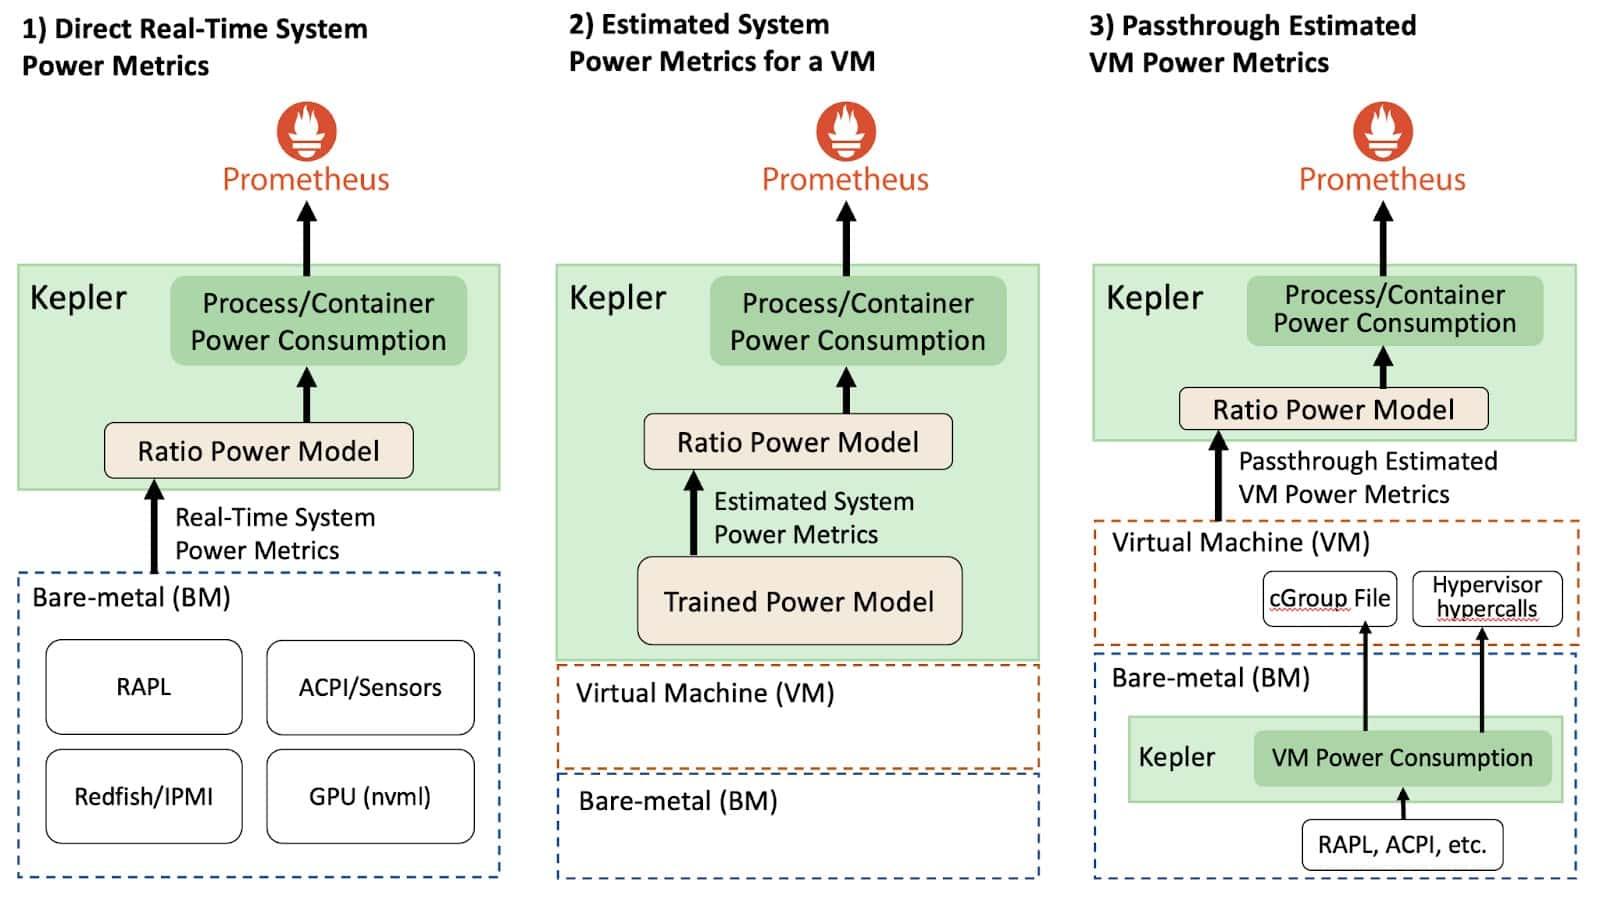
\includegraphics[width=0.8\textwidth]{Figures/kepler_deployment_modes.jpg}
  \caption{Kepler deployment models: direct power measurement on bare-metal, estimation on VMs, and the proposed passthrough model (currently not implemented).}
  \label{fig:kepler-deployment-modes}
\end{figure}

\paragraph{Kepler Agent and Exporter}
The core monitoring functionality is handled by the Kepler Agent, which is deployed as a privileged DaemonSet pod on each Kubernetes node. It collects resource utilization metrics using a combination of eBPF instrumentation and hardware performance counters exposed via \texttt{perf\_event\_open}. A kprobe attached to the \texttt{finish\_task\_switch} kernel function enables accurate tracking of per-process context-switch activity. Container and pod attribution is performed after parsing the cgroup path from \texttt{/proc/\$PID/cgroup} and querying the Kubelet API for container metadata. The generated metrics are exported via a Prometheus-compatible endpoint for downstream processing and visualization.

\begin{figure}[ht]
  \centering
  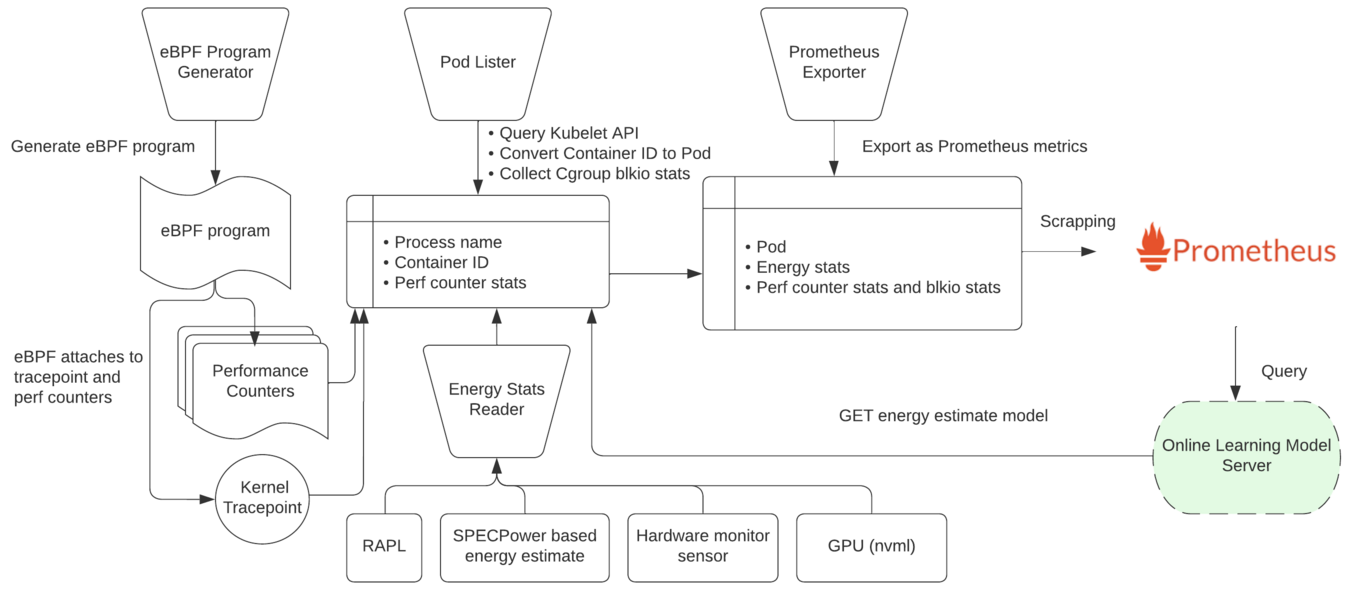
\includegraphics[width=0.8\textwidth]{Figures/kepler_architecture.png}
  \caption{Simplified architecture of the Kepler monitoring agent and exporter components.}
  \label{fig:kepler-architecture}
\end{figure}



xxxxxxxxxxxxxxxx



\paragraph{Metric Types and Sources}
Kepler collects a broad set of low-level metrics that form the foundation for power attribution. These include hardware performance counters such as CPU instructions, CPU cycles, reference cycles (not affected by scaling), and cache misses. In addition, eBPF-based probes are used to collect CPU time, block I/O, and network IRQ activity. All metrics are exposed as Prometheus counters, allowing power consumption to be computed as a rate of energy (Joules) over time using standard PromQL expressions (e.g., \texttt{irate()}).

\paragraph{Estimator Sidecar and Model Inference}
In addition to its lightweight internal estimator, Kepler optionally supports an estimator sidecar container that uses more sophisticated regression models for power inference. The sidecar communicates with the exporter via a Unix domain socket and loads pre-trained models (e.g., Scikit-learn, XGBoost) suitable for online estimation in environments lacking direct power metrics. This mechanism is mainly intended for telemetry-sparse environments and is not used in the real-time deployment mode considered in this thesis.

\paragraph{Model Server and Model Training}
For use cases requiring power estimation, Kepler includes a separate model server that can train energy models from Prometheus-collected metrics and power measurements. The training pipeline involves isolating dynamic power consumption using various strategies (e.g., pre-profiling or regression-based idle estimation) and applying regression techniques to fit models for node-level or component-level power. These models are then made available through a shared model repository. While model training plays a key role in estimation-only environments, it is not central to the goals of this thesis\parencite{choochotkaewAdvancingCloudSustainability2023}.

\paragraph{External Integration}
Kepler is designed to integrate seamlessly with existing observability tools. Prometheus is used to scrape metrics from the Kepler agent, and dashboards can be built using Grafana to visualize energy consumption across nodes, containers, or applications. While not required for the core functionality, this integration facilitates operational awareness and debugging.



% - High-level architecture: Exporter, Estimator, Model Server
% - Exporter: eBPF-based tracing, cgroup info, PID-to-container mapping
% - Metric sources:
%   - Utilization: CPU instructions, cycles, cache misses, IRQs
%   - Power: RAPL (sysfs/MSR), ACPI, IPMI/Redfish, NVML
% - Estimator sidecar: model selection and inference
% - Model Server:
%   - Trains regression models from Prometheus data
%   - Supports absolute (AbsPower) and dynamic (DynPower) modes
%   - Uses benchmark + isolator pipeline for training
% - RAPL for CPU and DRAM
% - ACPI for system power consumption
% - ebpf for performance counters (at the context-level switch)

% COMPONENTS:
% - KEPLER Agent: Core monitoring agent that runs on each node, collects metrics via eBPF, cgroups, etc., and (optionally) estimates energy usage using power models
% - KEPLER Exporter: Exposes metrics via Prometheus (both raw system metrics and estimated power consumption)
% - KEPLER Model Server: Central service to train and serve power estimation models using usage metrics + power labels (e.g., RAPL)
% - KEPLER Model DB: Repository of pre-trained power models (e.g., trained on SPECpower, nx12 workloads)
% - KEPLER Estimator (Sidecar): An optional sidecar container that uses the general estimator (e.g., scikit-learn models) instead of just the lightweight local linear estimator
% - Prometheus + Grafana (External)	Used to scrape metrics from Kepler and visualize them


% - designed to be extensible
% - provides integratesd view of node power consumptino across different resources and modes.
% - promotes fair distribution o f system pwoer consumption on the basis of the Green House Gas (GHG) Protocol\parencite{gesi2024ictguidance}.
%     includes separation of idle power and any overhead based on allocated capacity, as well as dynamic power based on utilization.

% Components:
% - Metric exporter (module)
%     uses a BPF program to extract process-related metrics. Also collects real-time power metrics (RAPL, ACPI, ...) using perf\_events functions of BPF to retrieve hardware counter information.
%     for each BPF program, the PID of the last thread in kernel space is stored.
%     The container ID is determined by scanning /proc/\$PID/cgroug. Using the containerID, the pod info (name/namespace) is retrieved through Kubelet Container API
%     the module alsp performas a calibration phase to discover idle and activation power in the server as part of the training workflow
%     the collected data is periodically sent to the model server module for training the power model

% - Model server (module)
%     responsible for training the power model for each node using the data collected during the training phase
%     determine model parameters
%     IMPORTANT: the idea of these models is to accurately estimate energy consumption in the ABSENCE of power data, having used them as ground truth for training.
%     implemented in python -> strong support for statistical libraries (e.g. Scikit-learn, XGBoost, PyGam) to hanle regression models

% - Energy Inference (module) (not mentioned often)
%     uses power model parameters and aggregated metrics to calculate power consumption at process level



\subsubsection{Attribution Model and Output}
\label{sec:kepler-attribution}
% - Ratio Power Model:
%   - Dynamic power → attributed by usage ratio
%   - Idle power → split by container size (GHG Protocol)
% - Container-level metrics (e.g., kepler_container_joules_total)
% - Node-level aggregation
% - Metric types: core, dram, uncore, package, gpu, other
% - Prometheus integration, usage of rate()/irate() for power
"our approach ensures the fair distribution of constant power among the user’s processes."
3 CATEGORIES:
- idle: minimum power of system at rest / background: minimum power of all background processes
- dynamic constrant: "activated by initial processes and remains constant regardless of load: "activation power"
- dynamic variable: solely dependent on resource utilization: "load-dependent power"

% - Processes not in a kubernetes or libvirt domain are identified as system_processes or kernel\_processes
"self-calibrating and extensible"

\subsubsection{Validation and Research Context}
\label{sec:kepler-validation}
% - Amaral et al.: improved MSE with process-level training
% - Use in other research (e.g., Gudepu, Soldani)
% - Evaluation by Pijnacker:
%   - Partial accuracy at node level
%   - Issues with idle attribution, system process inflation
% - Model validation challenges: hardware-specific, no ground-truth for containers
% - Adoption beyond Kepler (e.g., CLEVER, PEAKS)
- a short power model accuracy validation is done in the original KEPLER paper:
    CPU time leads to better accuracy than CPU cycles, (further investigation is necessary)
    but generally, more metrics always improve accuracy
    esults indicate that Linear regression did not yield satisfactory outcomes after incorporating cache and branch miss metrics


Detailed Validation by Pijnacker\parencite{pijnackerEstimatingContainerlevelPower2024, pijnackerContainerlevelEnergyObservability2025}
--> DO AFTER

\subsubsection{Limitations and Open Issues}
\label{sec:kepler-limitations}
% - Inaccuracy in container-level attribution (esp. idle power)
% - VM limitations:
%   - No access to real-time metrics
%   - Overestimation due to lack of host context
% - Pre-trained model issues: hardware-specific, lack of transferability
% - Overhead concerns: eBPF sampling, Prometheus scraping
% - Ongoing/future work:
%   - Multi-level deployment (BM → VM)
%   - Adaptive sampling, model filtering, vendor-agnostic support




































\subsection{Scaphandre}
\label{sec:scaphandre}

\subsubsection{Overview and Goals}
\label{sec:scaphandre-overview}

Scaphandre\parencite{scaphandre_github} is an energy monitoring agent designed to expose power consumption metrics at fine granularity, particularly in containerized and virtualized environments. Its name, derived from the French word for "diving suit" reflects its goal of providing deep insights into system-level energy consumption.

Scaphandre aims to attribute energy usage to individual processes, containers, or pods. It supports multiple deployment models: it can be installed directly on a physical host (where it can also monitor qemu/KVM-based virtual machines) or deployed in a container, measuring the energy usage of the host system, provided that the \texttt{/sys/class/powercap} and \texttt{/proc} directories are mounted as volumes. Most relevant to this thesis, Scaphandre can also be deployed on a Kubernetes cluster via a Helm chart, optionally alongside \textit{Prometheus} and \textit{Grafana}, allowing for convenient monitoring of Kubernetes nodes and containers.

\subsubsection{Architecture and Metric Sources}
\label{sec:scaphandre-architecture}

Scaphandre is written in Rust and features a modular, extensible architecture built around two core components: \textit{sensors} and \textit{exporters}. Sensors gather energy-related data from the host system, while exporters format and expose this data to external systems. This design allows seamless integration into cloud-native observability stacks and automation pipelines.

\paragraph{\textit{Sensors}}

Scaphandre’s \textit{Sensors} subsystem collects utilization and energy consumption metrics from the host system and makes them available to exporters. An abstraction layer, implemented in \texttt{sensors/mod.rs}, manages system topology (tracking sensors, CPU sockets, RAPL domains, and processes) and manages the generation of metric records.

The default Linux implementation, \texttt{PowercapRAPLSensor} (located in \texttt{powercap\_rapl.rs}), constructs a power topology by reading Intel RAPL data from the \texttt{/sys/class/powercap} interface. By default, it identifies all available domains (across all sockets) by matching directories with the pattern \texttt{intel-rapl:<socket>:<domain>}, each containing a domain name and an \texttt{energy\_uj} file reporting cumulative energy in microjoules. If no domain-level directories are found, Scaphandre triggers a fallback mechanism that omits subdomain detail and instead reads from the socket-level file, if available. This file represents the \texttt{package} (PKG) domain, which aggregates the energy consumption of the entire CPU socket. While PKG is a standalone RAPL domain, it also serves as the root of the domain hierarchy. Notably, Scaphandre does not currently handle overflow in the \texttt{energy\_uj} counter, a known limitation that has not yet been resolved despite user-reported inaccuracies~\cite{scaphandre_issue280}.

In addition to the Powercap-based sensor, a Windows-only sensor is available that reads energy consumption directly from Intel or AMD-specific Model-Specific Registers (MSRs).

System utilization metrics are collected by helper functions implemented in \texttt{utils.rs}, which rely on Rust’s \texttt{sysinfo} and \texttt{procfs} crates. These libraries extract data from virtual filesystems such as \texttt{/proc}, \texttt{/sys}, and \texttt{/dev}. When container support is enabled, cgroups are also read—but solely to map processes to containers. The collected metrics are stored in a custom data structure along with timestamps, while cgroup information is attached to each process as additional metadata labels. Apart from metrics of processes, CPU and memory, disk read/write operations are also collected.

The \textit{sensors} abstraction layer also applies key data preprocessing steps with are discussed in section ~\ref{sec:scaphandre-attribution}.

\paragraph{\textit{Exporters}}
\textit{Exporters} are responsible for collecting metrics from sensors, storing them temporarily, and exporting them to external systems. Crucially, they also perform the attribution of energy and system metrics to specific scopes, which is discussed in detail in the following section. Similar to the sensor subsystem, Scaphandre uses an abstraction layer (implemented in \texttt{exporters/mod.rs}) to manage common exporter logic such as metric preparation and attribution. Individual exporters are implemented as pluggable modules and operate on a shared core. The \texttt{MetricGenerator} plays a central role by consolidating and attributing metrics across all scopes: the Scaphandre agent itself, the host, CPU sockets, RAPL domains, system-wide statistics, and individual processes.

The modular exporter architecture enables easy implementation of new output formats, and Scaphandre explicitly encourages developers to implement custom exporters if needed. Currently, exporters exist for \textit{Prometheus}, \textit{Stdout}, \textit{JSON}, and \textit{QEMU}, among others.

The \textit{QEMU} exporter is particularly notable. It is designed for use on QEMU/KVM hypervisors and allows energy metrics to be exposed to virtual machines (VMs) in the same way that the \texttt{powercap} kernel module does on bare-metal systems. Specifically, the QEMU exporter writes VM-specific energy metrics to a virtual file system. Inside the VM, a second Scaphandre instance can read these files as if they were native energy interfaces. This mechanism mimics a bare-metal powercap environment, allowing software running in the VM to access energy data without direct access to RAPL or hardware sensors. This architecture is especially useful for breaking the opacity of power monitoring in virtualized environments, where such metrics are usually unavailable. If adopted by cloud providers, this could significantly improve visibility into energy consumption within public cloud VMs, supporting energy-aware software design even in virtualized infrastructures.

\paragraph{Measurement Interval}
Scaphandre's measurement interval is fixed at two seconds, as defined in the \texttt{show\_metrics} function of the file \texttt{/exporters/prometheus.rs}. This hardcoded interval determines how frequently the agent performs a new measurement by reading cumulative energy values from the RAPL interface. While RAPL counters are updated approximately every millisecond, Scaphandre does not take advantage of this high-resolution data. Reducing the interval could improve measurement accuracy and temporal granularity (especially for short-lived processes) but would also increase system overhead. As of now, modifying the interval would require changes to the source code.

\subsubsection{Attribution Model}
\label{sec:scaphandre-attribution}

Scaphandre attributes power consumption to processes and containers using a proportional model based on CPU usage over time. At each sampling interval, it reads the system's total energy consumption from Intel RAPL counters and distributes this energy among all active processes according to their normalized CPU utilization.

The core of this attribution logic is based on CPU time as reported in \texttt{/proc}. For each process, Scaphandre accumulates CPU time in active states and excludes time spent in inactive states such as \texttt{idle}, \texttt{iowait}, \texttt{irq}, and \texttt{softirq}. This filtering is applied both at the per-process and system level, so that only time considered "active" is included in the normalization denominator. The result is a time-based utilization model that excludes idle-related CPU time from consideration.

Per-process energy is then computed using the following formula, conceptually implemented in \texttt{get\_process\_power\_consumption\_microwatts()}:
\begin{equation}
E_{\text{proc}}(t) = \frac{E_{\text{RAPL}}(t) \cdot \text{CPU}_{\text{proc}}(t)}{\sum_i \text{CPU}_i(t)}
\end{equation}
where \( E_{\text{RAPL}}(t) \) denotes the energy delta over the sampling interval \( t \), and \( \text{CPU}_{\text{proc}}(t) \) is the active CPU time of the process. The denominator includes the sum of active CPU time across all processes, excluding inactive states.

Container-level attribution is achieved by inspecting the cgroup path of each process and mapping it to a container or Kubernetes pod using runtime-specific metadata. When container context is available, Scaphandre enriches its per-process metrics with labels such as \texttt{container\_id}, \texttt{kubernetes\_pod\_name}, and \texttt{namespace}. These metrics, such as \texttt{scaph\_process\_power\_consumption\_microwatts}, are then exposed via Prometheus and can be aggregated at container or pod level.

In addition to process- and container-level metrics, Scaphandre also reports host-level power consumption using the \textit{PSYS} RAPL domains. These host metrics include total platform or package energy consumption, as available, and are exposed via metrics such as \texttt{scaph\_host\_power\_microwatts} and \texttt{scaph\_host\_energy\_microjoules}. Notably (as pointed out in section~\ref{sec:RAPL}), the \textit{PSYS} domain typically does not exist on server-grade systems, in which case Scaphandre adds the \textit{PKG} and \textit{DRAM}-packages to calculate host consumption. Unlike per-process energy values, these host-level metrics reflect total system energy use and are not adjusted to exclude idle CPU time.

\paragraph{Idle power consumption}
Scaphandre does not compute idle power directly, but it is possible to infer a residual estimate by comparing the total reported host power to the sum of per-process power:
\[
P_{\text{idle}} = P_{\text{Host}} - \sum P_{\text{proc}}
\]
This difference may include contributions from idle power, system activity outside of user processes, or RAPL domain coverage gaps. However, this value is not part of Scaphandre’s exported metrics and must be computed externally if needed.

This attribution methodology is used consistently across the Scaphandre exporters, including the Prometheus exporter. It forms the basis for container-aware energy attribution without requiring additional instrumentation or hardware performance counter support. Further discussion of this methodology’s strengths, assumptions, and limitations follows in the next section.

\subsubsection{Validation and Research Context}
\label{sec:scaphandre-validation}

To date, no formal validation of Scaphandre’s attribution methodology has been published. While the underlying RAPL interface used for energy measurement is widely accepted and validated in prior research, the specific proportional attribution model employed by Scaphandre has not been systematically evaluated against ground-truth data or instruction-based models.Despite this, Scaphandre has been used in academic and applied contexts for estimating the energy consumption of software systems. In most cases, it is treated as a black-box exporter of container-level energy metrics, with limited investigation into its internal measurement and attribution logic.

A more detailed assessment is presented by Tarara\parencite{Tarara2023CpuUtilization}, who compares Scaphandre’s reported per-process power consumption against both CPU utilization and instruction-based measurements. His case study reveals that Scaphandre tends to overestimate power consumption for lightweight processes under low-load conditions, due to its policy of distributing all observed energy among the small set of active processes. While the model excludes idle time from CPU usage calculations, it does not exclude idle power from total energy, leading to attribution artifacts. Tarara concludes that Scaphandre improves upon naïve utilization-based models, but cannot match the precision of instruction-level approaches using tools such as \texttt{perf}.

\subsubsection{Limitations and Open Issues}
\label{sec:scaphandre-limitations}

While Scaphandre offers a lightweight and transparent approach to energy attribution, several limitations emerge from its current implementation.

First, its fixed measurement interval of 2 seconds limits temporal resolution. Although the underlying RAPL interface supports much finer granularity, Scaphandre aggregates CPU activity over 2-second windows. During this time, the Linux scheduler may switch between dozens or hundreds of processes, depending on system activity. As a result, Scaphandre can only attribute energy based on average CPU utilization over the interval, potentially masking short-lived or bursty behavior.

Second, Scaphandre attempts to refine CPU-based attribution by subtracting inactive time (\texttt{idle}, \texttt{iowait}, \texttt{irq}, \texttt{softirq}) from the denominator of its proportional model. While this adjustment excludes clearly non-active states, it does not fully resolve the underlying ambiguity of CPU utilization as a proxy for energy. As noted by Tarara\parencite{Tarara2023CpuUtilization}, when overall system load is low, the total observed energy (especially idle platform power) is still fully distributed among a small set of active processes. This can result in inflated or misleading per-process energy values, particularly for lightweight workloads.

Scaphandre relies exclusively on Intel’s RAPL interface for energy measurements. The developers of Scaphandre acknowledge the lack of detailed public documentation, especially for the \texttt{PSys} domain, which they assume to represent total SoC power. Their experiments also highlight ambiguity regarding domain overlaps—for instance, whether the \texttt{DRAM} domain is already included in \texttt{PKG}, or whether it must be treated as a separate component. These uncertainties may affect the interpretation of host-level energy metrics and the completeness of total system energy accounting.

In a comparison experiment between Scaphandre and other tools, Raffin\parencite{raffin2024dissecting} was unable to push scaphandres measurement frequency beyond 28 Hz, indicating a suboptimal implementation. Despite being written in Rust, Scaphandre performed significantly worse than the python-based tool \textit{CodeCarbon}. Raffin measured Scaphandre's overhead at a non-negligible 3-4\% at 10 Hz on an Intel Server.

Finally, Scaphandre does not incorporate instruction-level or performance counter-based metrics. It cannot distinguish between processes with different execution intensities or memory behavior, and assumes a uniform relationship between CPU time and energy use. This limits its ability to reflect differences in instruction throughput, stalling, or architectural efficiency across workloads.

\subsection{SmartWatts}
\label{sec:smartwatts}
\subsubsection{Overview and Goals}
\label{sec:smartwatts-overview}
The PowerAPI-implementation \textit{SmartWatts}\parencite{fieni2020smartwatts} is a software-defined, self-calibrating power 'formula' designed for estimating power consumption of containers, processes, and VMs. It aims to address the shortcomings of static power models by using online model adaptation (sequential learning) and runtime performance counters. Unlike many academic models that require manual calibration or architecture-specific training, SmartWatts adapts automatically to the host system and workload.
\subsubsection{Architecture and Metric Sources}
\label{sec:smartwatts-architecture}
SmartWatts is written in Pyhton. Understanding the architecture of SmartWatts and its differences from other energy monitoring tools is crucial. Using HWPC, RAPL, and CPU process metrics, SmartWatts collects performance data. At runtime, it uses power models based on cgroups and perf events alone to estimate, for each resource $\text{res} \in \{\text{CPU}, \text{DRAM}\}$, the host power consumption $\hat{p}_{\text{res}}$ and the power consumption $\hat{p}_{\text{res}}(c)$ for all containers. SmartWatts uses $\hat{p}_{\text{res}}$ to continuously assess the accuracy of the managed power models $M_{\text{res}, f}$ to ensure that estimated power consumption does not diverge from the RAPL baseline measurement $p_{\text{res}}^{\text{rapl}}$. When the estimation diverges beyond a configurable threshold $\epsilon_{\text{res}}$, SmartWatts triggers a new online calibration process for the model. When the machine is at rest (e.g., after a reboot), this method is also used to isolate the static energy consumption. A simple architecture can be seen in Figure~\ref{fig:smartwatts_architecture}.

In practical terms, SmartWatts implements a server-side pwoermeter (referred to as \textit{power meter}) that consumes input samples and produces power estimations accordingly. The power meter is responsible for power modelling, power estimation and model calibration. In addition, a client-side sensor (referred to as \textit{sensor}) is deployed as a lightweight daemon on all cluster nodes. The sensor is responsible static power isolation, event selection, cgroups and event monitoring. This separation allows for heterogeneous cluster nodes.

\begin{figure}[ht]
    \centering
    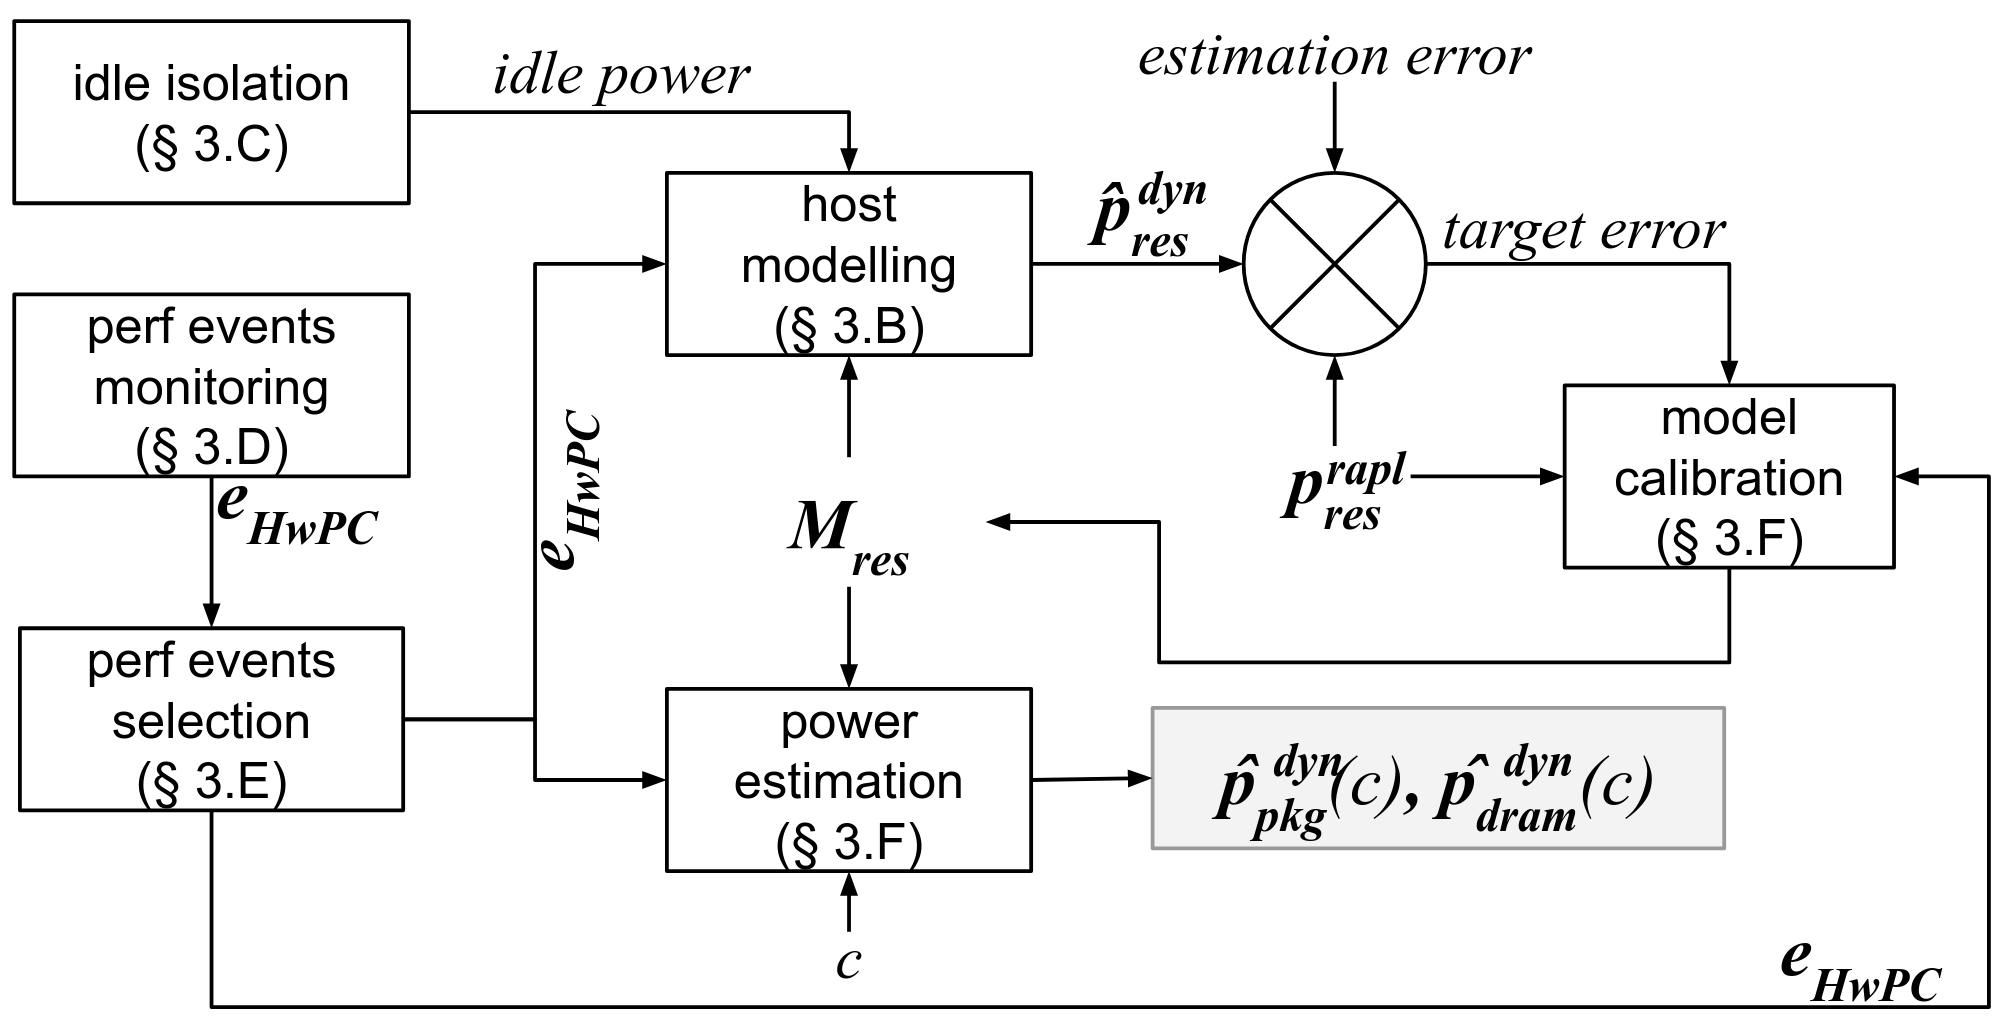
\includegraphics[width=0.7\textwidth]{Figures/smartwatts_architecture.png}
    \caption[SmartWatts architecture]{SmartWatts Architecture}
    \label{fig:smartwatts_architecture}
\end{figure}
\subsubsection{Attribution Model}
\label{sec:smartwatts-attribution}
As discussed in the previous subsection, the SmartWatts attribution model does not use RAPL metrics, opting only for process metrics. SmartWatts separates host energy consumption into static and dynamic power consumption:
\begin{equation}
    p_{res}^{rapl} = p_{res}^{static} + p_{res}^{dynamic}
\end{equation}

\textbf{Static power} is estimated by periodically logging RAPL package and DRAM power consumption. The $median$ value and the $interquartile range$ (IRQ) are gathered from teh measurements to define the static host power consumption as 
\begin{equation}
    p_{res}^{static} := median_{res} - 1.5 \cdot IRQ_{res}
\end{equation}
This approach is meant to filter out RAPL outliers.

\textbf{Dynamic power} is estimated by correlating the CPU frequency $f$ and the raw metrics reported by HWCP:
\begin{equation}
    \exists f \in F, \hat{p}_{res}^{dyn} = M_{res}^{f} \cdot E_{res}^{f}
\end{equation}
where $E_{res}^{f}$ denotes all \textit{events}. The model $M_{res}^{f}$ is build from \textit{elastic net} regression applied on the last $k$ samples. To ensure that all container power consumptions are linear with regards to global power consumption, positive inference coefficients are enforced, and the intercept (or \textit{bias term} is within the range $[0, TDP]$.

\textbf{HWPC metrics} are dynamically chosen based on the list of available events exposed by the host's \textit{Performance Monitoring Units} (PMU), essentially creating a custom model based on available metrics. Not all available metrics are used, and statistical analysis (Pearson coefficient) is used to determining worthy candidates.

\textbf{Container power consumption} is estimated by applying the inferred power model $M_{res}^{f}$ at the scale of the container's events $E_{res}^{f}(c)$, as seen in formula~\ref{for:smartwatts_container_events}. In formula~\ref{for:smartwatts_container_intercept}, the intercept $i$ is distributed proportionally to the dynamic part of the consumption of $c$.
\begin{equation}
\label{for:smartwatts_container_events}
    \exists f \in F, \forall c \in C, \hat{p}_{res}^{dyn}(c) = M_{res}^{f} \cdot E_{res}^{f}(c)
\end{equation}
\begin{equation}
\label{for:smartwatts_container_intercept}
    \forall c \in C, \tilde{p}_{res}^{dyn}(c) = \hat{p}_{res}^{dyn}(c) - i \cdot (1-\frac{\hat{p}_{res}^{dyn}(c) -i}{\hat{p}_{res}^{dyn} -i})
\end{equation}

In theory, one can expect $\hat{p}_{res}^{dyn} \overset{!}{=} {p}_{res}^{dyn}$ if the model perfectly estimates the dynamic power consumption, but in practice, an error $\epsilon_{res} = \left| {p}_{res}^{dyn} - \hat{p}_{res}^{dyn} \right|$. Therefore, container power consumption is capped at
\begin{equation}
    \forall c \in C, \left\lceil \tilde{p}_{res}^{dyn}(c) \right\rceil = \frac{{p}_{res}^{dyn} \cdot \tilde{p}_{res}^{dyn}(c)}{\hat{p}_{res}^{dyn}}
\end{equation}
This approach also allows to calculate a confidence intercal of the power consumption of containers by scaling down the observed global error:
\begin{equation}
    \forall c \in C, \epsilon_{res}(c) = \frac{\tilde{p}_{res}^{dyn}(c)}{\hat{p}_{res}^{dyn}} \cdot \epsilon_{res}
\end{equation}

In order improve estimation accuracy, the following configurable parameters are used:
\begin{itemize}
    \item CPU-TDP in Watt (default: 125)
    \item CPU base clock in MHz (default: 100)
    \item CPU base frequency in MHz (default: 2100)
    \item CPU and DRAM error threshold in Watt (default: 2)
    \item Minimum of samples required before trying to learn a power model (default: 10)
    \item Size of the history window used ot keep samples from (default: 60)
    \item Measurement frequency in milliseconds (default: 1000)
\end{itemize}
\subsubsection{Validation and Research Context}
\label{sec:smartwatts-validation}
With RAPL being used as ground truth for dynamic power estimation model recalibration, it is important to note that the SmartWatts validation is focused on the model accuracy when compared to RAPL values instead of values obtained by an external source of power data. The SmartWatts validation focused on the quality of power estimation in sequential and parallel workloads, the accuracy and sstability of power models and the overhead of the \textit{sensor} component. Standard benchmarks like Stress-NG and NAS parallel Benchmarks were chosen. 

While there is no advanced statistical analysis, the validation shows that, for a error threshold for CPU and DRAM of 5 and 1 Watt respectively, power consumption can be reliably estimated with less than 3 Watts and 0.5 Watts, respectively. The only case where the error grows beyond the threshold is at the CPU idle frequency. The model stability is shown to significantly improve when lower recalibration frequencies are used. SmartWatts succeeds to reuse a give power model for up to 594 estimations, depending on frequency. The monitoring overhead is observed to be at 0.333 Watts for the PKG domain and 0.030 Watts for the DRAM domain on average, at a measurement frequency of 2 Hz. The authors consider this overhead negligable.
\subsubsection{Limitations and Open Issues}
\label{sec:smartwatts-limitations}
SmartWatts offers a compelling solution for dynamic, container-level power estimation through self-calibrating models based on performance counters. However, its applicability remains domain-specific. The central assumption is that RAPL, while accurate, is too coarse-grained for attributing power to individual containers or processes. This premise is debatable: RAPL offers low-overhead, high-frequency measurements, and may be sufficient for many use cases, particularly in homogeneous or single-tenant systems. Whether SmartWatts' added complexity is justified depends on how fine-grained the attribution needs to be.

SmartWatts shines when more granular telemetry (e.g., perf events) is available and container-level attribution is critical. Yet its current implementation models only CPU and DRAM domains, limiting its ability to offer a comprehensive energy profile.

The design allows operators to supply hardware-specific values (e.g. CPU TDP), while falling back to sensible defaults. This improves usability without sacrificing model accuracy.

Finally, while SmartWatts' runtime calibration and dynamic event selection enhance adaptability, they introduce complexity. The event selection mechanism relies on statistical heuristics, which may not generalize well across systems. Moreover, under highly dynamic conditions, frequent recalibrations may affect stability.

In summary, SmartWatts is well-suited for environments requiring high-resolution attribution beyond RAPL's capabilities, but its scope, complexity, and assumptions warrant careful consideration depending on the target use case.


\section{Comparison of Container-Level Tools}
\label{sec:tool-comparison}
\subsection{Feature Comparison}
\label{sec:feature-comparison}
\subsection{Granularity and Metric Sources}
\label{sec:granularity-comparison}
\subsection{Platform Compatibility and Integration}
\label{sec:integration-comparison}

\section{Relevance to Proposed Architecture}
\label{sec:relevance-to-architecture}
\subsection{Lessons Learned from Existing Tools}
\label{sec:lessons-learned}
\subsection{Identified Gaps and Opportunities}
\label{sec:tool-gaps}
\subsection{Implications for Chapter \ref{chap:architecture}}
\label{sec:implications-architecture}

\section{Summary}
\label{sec:tool-summary}




\subsubsection{Overview and Architecture}
% What the tool does, where it runs, general design.
\subsubsection{Metrics and Data Sources}
% What it measures, how it collects (RAPL, perf, eBPF, etc.).
\subsubsection{Attribution Method and Scope}
% How power is assigned to tasks (processes, VMs, containers).
\subsubsection{Validation and Limitations}
% Is it validated? Known weaknesses or constraints?
\subsubsection{Relevance to Proposed Architecture}
% Optional – What ideas or drawbacks will influence your own model.



\begin{comment}
    4.1 Overview of Tool Landscape
        KEPLER, Scaphandre, CodeCarbon, PowerAPI, Cloud Carbon Footprint, etc.
    4.2 Tool Analysis Framework
        Accuracy, data sources, correlation method, platform support, etc.
    4.3 Detailed Evaluation of Selected Tools
        One subchapter per tool:
            4.X KEPLER
            4.X Scaphandr
            ...
    4.4 Comparison Summary
        Table of tradeoffs
        Strengths and weaknesses
        Missing features / open gaps


\section{Tools}
\subsection{RAPL-based tools}
\label{sec:rapltools}
\begin{itemize}
    \item \parencite{jay2023experimental} An experimental comparison of software-based power meters (focus on CPU / GPU)
    \item \parencite{van2025powersensor3} fast accurate opensource: PowerSensor3 enables real-time power measurements of SoC boards and PCIe cards, including GPUs, FPGAs, NICs, SSDs, and domain-specific AI and ML accelerators
    \item \parencite{scaphandre_documentation} Scaphandre. Does not handle overflows correctly (https://github.com/hubblo-org/scaphandre/issues/280)
    \item \parencite{fieni2020smartwatts} Smartwatts: Self-Calibrating Software-Defined Power Meter for containers
    \item \parencite{joularjx} JoularJX: java-based agent for power monitoring at the code level
    \item \parencite{kepler_energy}: KEPLER
    \item \parencite{powertop}: powertop
    \item \parencite{greencodingdocs}: Green metrics tool: measuring energy and CO2 consumption of software through a software life cycle anslysis (SLCA): Metric providers: RAPL, IPMI, PSU, Docker, Temperature, CPU, ... (sone external devices)
    
    % according to raffin2024: simplified versions of scaphandre and codecarbon hhve 3\%, 0.5\% overhead at 10Hz
    % according to \parencite{jay2023experimental}, the full versions have between 2 and 7\% at 1Hz.

    powerAPI            Focuses on per-process measurement, not container nor Kubernetes aware
    WattsUpDoc          Focuses on data center-wide telemetry, not container-level granularity
    Perf/EnergyPerf     Offers per-core/per-task telemetry, but requires extensive integration to map to containers
    PowerTOP            Local profiling tool; not suited for cluster-wide telemetry or Kubernetes
    PowerAPI -> on github contains repos for powerapi, smartwatts-formula, hwpc-sensor, pyjoules
    EnergyVisor
    nvme-cli
    PAPI (uses RAPL)


\parencite{fieni2024powerapi}: PowerAPI: Python framework for building software-defined power
\end{itemize}

- multiple papers have tried to attribute component-level 




\section{Container-Level Monitoring Tools}
    KEPLER, Scaphandre, Smartwatts, JoularJX, AI Power Meter, CodeCarbon.
    Granularity down to the container level.
    internal mechanisms (e.g., eBPF, RAPL, NVML).
    Advantages and drawbacks.
    
\section{Comparison of Tools}
    Detailed matrix comparing:
        Measurement methodology.
        Component focus (CPU, RAM, GPU, Disk, Network).
        Real-time capabilities.
        Kubernetes compatibility.
\end{comment}